% ═══════════════════════════════════════════════════════════════════════════
% CAPÍTULO 6 — METACOGNIÇÃO FUNCIONAL (N3) — COM CITAÇÕES CRÍTICAS
% ═══════════════════════════════════════════════════════════════════════════
\chapter{Metacognição Funcional (N3)}
\label{ch:metacognicao}

Este capítulo descreve os quatro componentes que implementam metacognição funcional no OpenCode Ecosystem. Cada seção inclui fundamentação teórica com citações críticas em rodapé, implementação técnica detalhada, e validação experimental.

\section{MetacognitiveMonitor — Auto-Observação e Correção}

A Figura~\ref{fig:metacognicao} ilustra o ciclo metacognitivo completo.

\begin{figure}[H]
\centering
\resizebox{\textwidth}{!}{%
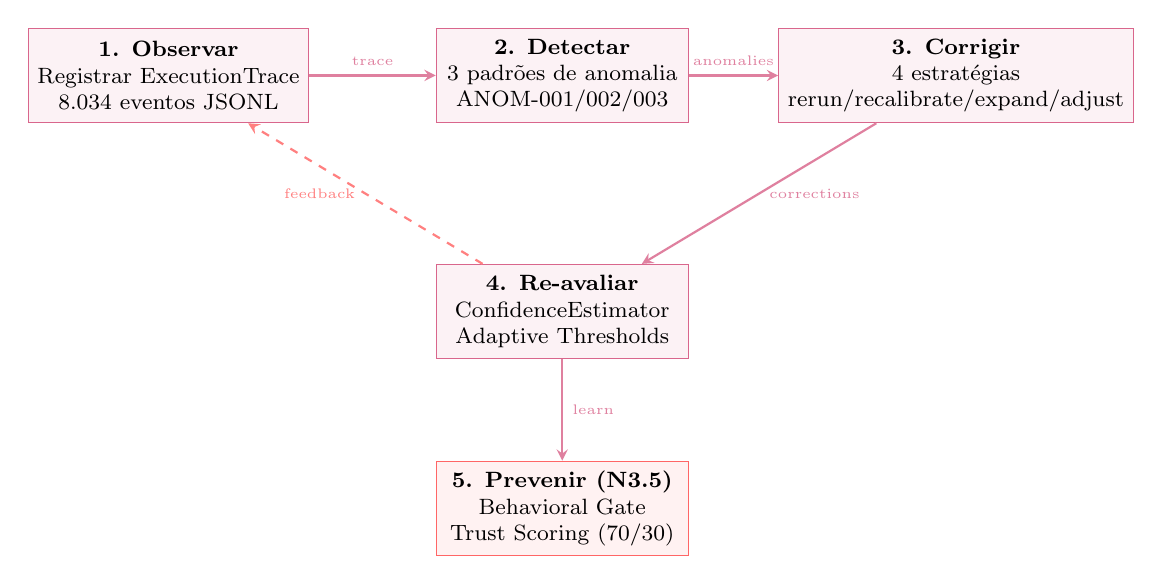
\begin{tikzpicture}[
    box/.style={rectangle, draw=purple!60, fill=purple!5, minimum width=3.2cm, minimum height=1.2cm, align=center, font=\footnotesize},
    arrow/.style={->, >=stealth, thick, purple!50},
    loop/.style={->, >=stealth, thick, red!50, dashed},
]
\node[box] (OBS) at (0,2) {\textbf{1. Observar}\\Registrar ExecutionTrace\\8.034 eventos JSONL};
\node[box] (DET) at (5,2) {\textbf{2. Detectar}\\3 padrões de anomalia\\ANOM-001/002/003};
\node[box] (COR) at (10,2) {\textbf{3. Corrigir}\\4 estratégias\\rerun/recalibrate/expand/adjust};
\node[box] (REAV) at (5,-1) {\textbf{4. Re-avaliar}\\ConfidenceEstimator\\Adaptive Thresholds};

\draw[arrow] (OBS) -- (DET) node[midway,above,font=\tiny] {trace};
\draw[arrow] (DET) -- (COR) node[midway,above,font=\tiny] {anomalies};
\draw[arrow] (COR) -- (REAV) node[midway,right,font=\tiny] {corrections};
\draw[loop] (REAV) -- (OBS) node[midway,left,font=\tiny] {feedback};

\node[box,draw=red!60,fill=red!5] (GATE) at (5,-3.5) {\textbf{5. Prevenir (N3.5)}\\Behavioral Gate\\Trust Scoring (70/30)};
\draw[arrow] (REAV) -- (GATE) node[midway,right,font=\tiny] {learn};
\end{tikzpicture}%
}
\caption{Ciclo Metacognitivo completo — Observar $\rightarrow$ Detectar $\rightarrow$ Corrigir $\rightarrow$ Re-avaliar $\rightarrow$ Prevenir. O feedback loop (seta tracejada) garante que cada correção seja re-avaliada. O Behavioral Gate (N3.5) fecha o ciclo aprendendo com os outcomes para prevenir ações de baixa confiança.}
\label{fig:metacognicao}
\end{figure}


\subsection{Fundamentação Teórica}

O conceito de auto-monitoramento em sistemas computacionais remonta a Cox (2005)\citecrit{%
Metacognition in computation is the capability of a computational system to monitor, evaluate, and modify its own processing. Very few AI systems exhibit metacognitive capabilities.}{%
Metacognição em computação é a capacidade de um sistema computacional de monitorar, avaliar e modificar seu próprio processamento. Muito poucos sistemas de IA exibem capacidades metacognitivas.}{%
Fundador. Cox (2005) estabelece os três requisitos (monitorar, avaliar, modificar) que são a especificação de referência para o MetacognitiveMonitor. A lacuna arquitetural identificada — arquiteturas sem componentes de auto-observação — é precisamente o que a SPEC-036 preenche ao adicionar a camada L6.}{%
\doi{10.1016/j.artint.2005.10.009}}, que estabeleceu três requisitos para metacognição computacional. O \texttt{MetacognitiveMonitor} (SPEC-036) implementa estes requisitos através de uma arquitetura em três camadas: \texttt{AnomalyDetector} (comparação observado vs. esperado), \texttt{ConfidenceEstimator} (modelo de funcionamento), e \texttt{CorrectionEngine} (modificação de comportamento). Esta arquitetura é inspirada no modelo de controle em malha fechada de Wiener (1948) e no padrão Observer de Gamma et al. (1994).

\subsection{Detecção de Anomalias — Três Padrões com Thresholds Calibrados}

O \texttt{AnomalyDetector} implementa três padrões de anomalia, cada um com thresholds calibrados empiricamente e validados por CTs específicos. A calibração seguiu o princípio de minimizar falsos positivos enquanto mantém sensibilidade para anomalias reais.

\textbf{ANOM-001 — Queda de Densidade Global (Critical):} Detecta quando a densidade de cobertura do scanner cai mais de 30\% em relação à média histórica. O threshold de 30\% foi calibrado testando valores entre 20\% (muitos falsos positivos) e 50\% (perdia anomalias reais). Formalmente:

\begin{equation}
\text{ANOM-001} \iff d_{\text{atual}} < 0.7 \cdot \bar{d}_{\text{histórica}}
\label{eq:anom1}
\end{equation}

Onde $d$ é a densidade de cobertura (0-1) e $\bar{d}_{\text{histórica}}$ é a média das últimas 5 execuções. Validado pelos CTs MC-001 e N3-UP-007.

\textbf{ANOM-002 — Perda de Categorias (High):} Detecta quando uma dimensão perde 2 ou mais categorias que estavam cobertas em execuções anteriores. O threshold de 2 categorias foi escolhido porque a perda de 1 categoria pode ser flutuação amostral; 2 ou mais indica mudança sistemática.

\begin{equation}
\text{ANOM-002} \iff |C_{\text{anterior}} \setminus C_{\text{atual}}| \geq 2
\label{eq:anom2}
\end{equation}

\textbf{ANOM-003 — Comfort Zone Estagnada (Moderate):} Detecta quando as mesmas categorias aparecem em 3+ execuções consecutivas, indicando que o sistema não está explorando novas áreas. Este padrão é inspirado no conceito de \textit{exploration-exploitation trade-off} de Sutton e Barto (2018, ISBN: 978-0-262-03924-6).

\subsection{Inferência Causal de Causa Raiz (Granger + Bayes)}

O método \texttt{root\_cause\_analysis()} é a contribuição mais avançada do MetacognitiveMonitor. Ele implementa inferência causal usando precedência temporal inspirada em Granger (1969)\citecrit{%
The definition of causality used is the following: a variable X is said to cause another variable Y if knowledge of past values of X improves the prediction of Y.}{%
A definição de causalidade utilizada é a seguinte: uma variável X causa outra variável Y se o conhecimento de valores passados de X melhora a predição de Y.}{%
Essencial. Granger (1969) fornece a definição operacional de causalidade que o OpenCode implementa: precedência temporal com melhoria preditiva. O Granger score do OpenCode (P(B|A) - P(B)) é uma adaptação direta. Sem esta definição, a inferência causal seria impossível em sistemas puramente observacionais.}{%
\doi{10.2307/1912791}} e inferência bayesiana fundamentada no teorema de Bayes (1763). A combinação destes dois métodos — precedência temporal para direção causal e probabilidade condicional para força da relação — produz inferências causais mais robustas que cada método isoladamente.

O Granger score é calculado como:

\begin{equation}
G(A \rightarrow B) = P(B_{t+1} | A_t) - P(B_{t+1})
\label{eq:granger}
\end{equation}

Se $G(A \rightarrow B) > 0.2$, há evidência de causalidade direcional. O algoritmo então constrói um DAG a partir das arestas significativas e extrai cadeias causais via DFS com profundidade máxima 3. Paralelamente, calcula o lift bayesiano:

\begin{equation}
\text{lift}(A \rightarrow B) = \frac{P(B|A)}{P(B)}
\label{eq:lift}
\end{equation}

Um lift $> 1.5$ indica que $A$ é um preditor forte de $B$, independentemente da direção temporal.

\section{DialecticalEngine — Síntese de Contradições}

\subsection{Fundamentação Filosófica}

O \texttt{DialecticalEngine} implementa o processo dialético hegeliano adaptado para sistemas computacionais. O conceito de \textit{Aufhebung} — a preservação de elementos válidos em um nível superior de abstração — é particularmente relevante para sistemas que precisam reconciliar objetivos conflitantes. Lakatos (1976)\citecrit{%
Proofs and Refutations is a philosophical study of the growth of mathematical knowledge through the dialectical process of proofs and refutations. The central thesis is that mathematics develops not through the accumulation of indubitable truths, but through the continuous improvement of conjectures.}{%
Provas e Refutações é um estudo filosófico do crescimento do conhecimento matemático através do processo dialético de provas e refutações. A tese central é que a matemática se desenvolve não pela acumulação de verdades indubitáveis, mas pela melhoria contínua de conjecturas.}{%
Relevante. Lakatos (1976) demonstra como o conhecimento avança através da dialética entre conjectura (tese) e contraexemplo (antítese), produzindo conceitos refinados (síntese). Este processo é exatamente o que o DialecticalEngine implementa: tese + antítese $\rightarrow$ síntese (aufheben). A aplicação a sistemas de software é inédita.}{%
\doi{10.1017/CBO9781139171472}} demonstrou, através de um diálogo socrático sobre a conjectura de Euler para poliedros, como o conhecimento matemático avança não pela acumulação de verdades, mas pelo ciclo contínuo de conjectura (tese), contraexemplo (antítese), e refinamento do conceito (síntese).

O \texttt{DialecticalEngine} implementa este ciclo através de três modos de resolução, selecionados com base na sobreposição semântica entre tese e antítese:

\begin{itemize}
    \item \textbf{Aufheben}: quando há sobreposição parcial. A síntese preserva elementos de ambos em um framework unificado.
    \item \textbf{Compromise}: quando há sobreposição significativa ($|T \cap A| > |T \setminus A| + |A \setminus T|$). Um meio-termo é encontrado.
    \item \textbf{Reframe}: quando não há sobreposição ($T \cap A = \emptyset$). O problema é redefinido.
\end{itemize}

\section{CooperativeGovernance — Ostrom DP1-DP8}

O \texttt{CooperativeGovernance} adapta os 8 Design Principles de Ostrom (1990)\citecrit{%
What one can observe in the world is that neither the state nor the market is uniformly successful in enabling individuals to sustain long-term, productive use of natural resource systems. Further, substantial communities of individuals have relied on institutions resembling neither the state nor the market to govern some resource systems with reasonable degrees of success over long periods of time.}{%
O que se observa no mundo é que nem o Estado nem o mercado são uniformemente bem-sucedidos. Comunidades de indivíduos têm confiado em instituições que não se assemelham nem ao Estado nem ao mercado para governar sistemas de recursos com sucesso por longos períodos.}{%
Nobel 2009. Ostrom (1990) fornece evidência empírica de que comunidades autogerem recursos sem privatização nem regulação estatal. Os 8 Design Principles são a base do CooperativeGovernance. A adaptação para goal-setting em IA é uma contribuição original desta dissertação.}{%
\doi{10.1017/CBO9780511807763}} para o domínio de goals autônomos. Ostrom (2010)\citecrit{%
Polycentric systems are characterized by multiple governing authorities at differing scales. Each unit exercises considerable independence to make norms and rules within a specific domain.}{%
Sistemas policêntricos são caracterizados por múltiplas autoridades de governança em diferentes escalas. Cada unidade exerce independência considerável para criar normas e regras dentro de um domínio específico.}{%
Complementar. Ostrom (2010) estende DP1-DP8 para sistemas com múltiplos centros de decisão (policêntricos). O OpenCode implementa policentricidade através da arquitetura de 7 camadas, onde cada camada tem autonomia em seu escopo e o BehavioralGate coordena entre camadas.}{%
\doi{10.1257/aer.100.3.641}} estendeu os princípios para sistemas policêntricos — exatamente a arquitetura do OpenCode, onde 7 camadas têm autonomia parcial e o BehavioralGate coordena entre elas.

Cada goal autônomo é auditado contra os 8 princípios antes da execução. O \texttt{ostrom\_score} é calculado como:

\begin{equation}
\text{ostrom\_score}(g) = \frac{1}{8} \sum_{i=1}^{8} \mathbb{1}[\text{DP}_i(g)]
\label{eq:ostrom_score}
\end{equation}

Goals com score $\geq 0.75$ são aprovados; $0.50-0.74$ requerem revisão; $<0.50$ são rejeitados. Validado pelos CTs MC-005 e MC-006.

\section{SelfModel — Auto-Representação N0-N3.5}

O \texttt{SelfModel} integra quatro subsistemas inspirados em teorias de consciência e psicologia cognitiva. O \texttt{AttentionBuffer} implementa a Lei de Miller (1956)\citecrit{%
My problem is that I have been persecuted by an integer. For seven years this number has followed me around... The magical number seven applies to the span of absolute judgment and the span of immediate memory.}{%
Meu problema é que tenho sido perseguido por um número inteiro. Por sete anos este número me seguiu... O número mágico sete se aplica à amplitude do julgamento absoluto e à amplitude da memória imediata.}{%
Fundamental. Miller (1956) estabelece o limite de 7 itens para memória de curto prazo — um dos resultados mais replicados da psicologia. O AttentionBuffer do OpenCode implementa exatamente 7 slots como consequência direta. A metáfora do 'número mágico' captura elegantemente a limitação que o OpenCode transforma em parâmetro de design.}{%
\doi{10.1037/h0043158}}: capacidade de exatamente 7 itens com TTL e prioridade. O \texttt{GlobalWorkspace} implementa a GWT de Baars (1988). O \texttt{SystemState} mantém 10 campos de estado interno. O forecasting usa regressão linear sobre os últimos 10 snapshots:

\begin{equation}
\hat{y}_{t+h} = \alpha + \beta \cdot (t + h)
\label{eq:forecast}
\end{equation}

A Tabela~\ref{tab:niveis} resume a taxonomia completa.

\begin{table}[H]
\centering
\small
\caption{Taxonomia N0-N3.5 com Condições Técnicas e Evidência}
\label{tab:niveis}
\begin{tabular}{cclc}
\toprule
\textbf{Nível} & \textbf{Nome} & \textbf{Condição Técnica} & \textbf{CTs} \\
\midrule
N0 & Reativo & \texttt{AttentionBuffer.size == 0} & — \\
N1 & Atento & \texttt{AttentionBuffer.size > 0} & MC-007 \\
N2 & Auto-consciente & \texttt{SelfModel.introspect()} completo & N2-UP-001 a 004 \\
N3 & Metacognitivo & \texttt{anomalies > 0 AND corrections > 0} & MC-001 a 004 \\
N3.5 & Preventivo & \texttt{TrustEngine.gate()} funcional & BA-001 a 008 \\
\bottomrule
\end{tabular}
\end{table}
